\documentclass[compsoc,conference,a4paper,10pt,times]{IEEEtran}
\IEEEoverridecommandlockouts
% The preceding line is only needed to identify funding in the first footnote. If that is unneeded, please comment it out.
% \usepackage{cite}
\usepackage{amsmath,amssymb,amsfonts}
\usepackage{algorithmic}
\usepackage{graphicx}
\usepackage{textcomp}
\usepackage{bmpsize}
\usepackage{xcolor}
\usepackage{lipsum}
% \usepackage[colorlinks=true,urlcolor=black,pdftitle="Type Flattening Obfuscation"]{hyperref}
\usepackage{hyperref}
\hypersetup{
  colorlinks = true,
  urlcolor = black,
  pdftitle = "Type Flattening Obfuscation",
  pdfauthor = "Ta Thanh Dinh"
}
\usepackage{tikz-cd}
\def\BibTeX{{\rm B\kern-.05em{\sc i\kern-.025em b}\kern-.08em
    T\kern-.1667em\lower.7ex\hbox{E}\kern-.125emX}}
\usepackage[sorting=ynt,sortcites=true,backend=bibtex8,doi=false,maxnames=6,isbn=false,firstinits=true]{biblatex}
\addbibresource{reference}

\begin{document}

\title{Type Flattening Obfuscation}

\author{\IEEEauthorblockN{Ta Thanh Dinh}
\IEEEauthorblockA{tathanhdinh@gmail.com}}

\maketitle

\begin{abstract}
  Beside data and control flow, high-level types are important in binary code analysis, particularly in
  decompilation. Some research papers have introduced methods to map machine-dependent objects into types
  of some C-like type system. For the obfuscation/anti-decompilation purpose, we
  present a technique which bypasses existing type recovery approaches. We have implemented a
  prototype obfuscating C compiler to demonstrate the technique, the compiler is
  given open source.
\end{abstract}

\begin{IEEEkeywords}
type recovery, decompilation, obfuscation
\end{IEEEkeywords}

\section{Introduction}
\noindent
Binary code \emph{decompilation}~\cite{cifuentes_reverse_1994} is to transform the low-level,
machine-dependent code of a program into a high-level form, like code of a high-level language.
In almost all academic research papers and commerical products, the target language is C.
Similar to compilers, a modern binary code decompiler consists of many
phases~\cite{cifuentes_reverse_1994,van_emmerik_static_2007}: disassembly, function boundary detection, immediate
representation (IR) lifting, control-flow graph (CFG) recovery, high-level variables detection,
type (i.e. variable types and function signatures) recovery, etc. Each phase requires
particular but not independent~\cite{schwarz_disassembly_2002} analysis techniques: the results of
one can affect another. The analyzed program is
transformed gradually into a higher-level, more abstract and more understandable representation.

In the opposite direction, binary code \emph{obfuscation} is a method to protect the low-level code from
being decompiled, or from being analyzed in general. Because the code analysis contains of different
interdependent phases, the obfuscation~\cite{banescu_tutorial_2018,collberg_surreptitious_2009}
can proceed at any of them, e.g. anti-disassembly
(binary packer, self-modifying code), binary stripping, control-flow flattening, virtualization (for both
data and control obfuscation)... just name a few. Basically, each obfuscation method consists of one or
several \emph{semantics-preserving} transformations~\cite{collberg_surreptitious_2009,dalla_preda_semantic-based_2005}
which hide certain properties of the code.

An optional feature of binary code decompilation is \emph{type reconstruction}, namely to recover high-level types from machine-dependent
objects~\cite{mycroft_type-based_1999, van_emmerik_static_2007}. This is the research objective of some
research papers~\cite{lee_tie_2011,elwazeer_scalable_2013,robbins_minx_2016,noonan_polymorphic_2016},
and killing feature of commercial~\cite{noauthor_hex-rays_nodate,noauthor_jeb_nodate}
as well as open source~\cite{noauthor_ghidra_nodate} binary code analysis tools. Beside decompilation,
types and particularly \emph{function signatures} are also essential in numerous applications,
e.g. static binary rewriting~\cite{bernat_anywhere_2011,anand_compiler-level_2013} and
raising~\cite{yadavalli_raising_2019},
see for example~\cite{caballero_type_2016} for a more completed list. Thus the knowledge about types
expand the attack surface since more analysis can be applied on the programs.

Despite of successes in binary type reconstruction and the need of protecting function signatures, to the best
of our knowledge there is no explicit effort in hiding type information. This paper presents a method
for type obfuscation, the principal idea is based on the fact that the compiler does not need to preserve all information
about high-level types (type erasure), then with specific tricks we can exploit the \emph{semantics gap} between
the high-level language and machine code to make some information very hard if not impossible
to be recovered. We do not claim that all type information can be hidden, the attacker can
eventually know some but it would be hard to distinguish the concrete underlying types from one to another,
thus the proposed notion of \emph{type flattening}.

We implement the tricks in \emph{uCc}, an open source obfuscating C compiler which obfuscates
function signatures. The functions in binaries generated by \emph{uCc} can be
perfectly analyzed by classical procedures (boundary detection, disassembling, CFG recovery, etc),
only their signatures are obfuscated. That way, we can evaluate the effectiveness of type
obfuscation tricks on function signatures while excluding unwanted obfuscation effects that may come from (bad) results
of other analysis phases.
We find that Mixed Boolean Arithmetic (MBA)
expressions~\cite{eyrolles_obfuscation_2017,zhou_information_2007} are a good match for the goal.

% \subsection*{Contributions}
% \noindent
In summary, our contributions are as follows:
\begin{itemize}
  \item We introduce the notion of \emph{type flattening}, it aims at protecting a high-level
  property (types) of the program in contrast with classical methods which focus on lower
  properties as data or control flow.

  \item We build a prototype compiler \emph{uCc} to realize the ideas of type
  flattening obfuscation. \emph{uCc} also implements the permutation polynomials
  of MBA~\cite{zhou_information_2007} while other open source state-of-the-art obfuscators
  (e.g. Tigress~\cite{noauthor_tigress_nodate}) give only basic arithmetic encoding expressions.
  Other deobfuscation tools (e.g. Syntia~\cite{blazytko_syntia_2017}, QSynth~\cite{david_qsynth_2020})
  can profit \emph{uCc} to test their capabilities of MBA simplification.

  \item We evaluate the binaries generated by \emph{uCc} against decent decompilers, the results
  show that no one can detect correctly the underlying types of arguments on function signatures: the
  original types are indistinguishable from the highest types in the C's integer conversion rank.
\end{itemize}

\section{Brief history of binary type inference}
\noindent
In statically typed languages, the compiler does not need preserve source code level type information in
the generated machine code (type erasure), then type recovering requires special techniques. A broad survey for research
up until 2015 can be referenced in~\cite{caballero_type_2016}, but it sustained a storage point of view bias: types are attached
always with some storage primitives (e.g. registers, memory), there are no essential differences between types and
data structures. Actually, types are compile-time constraints, they
may or may not have runtime storage imprints. An example is C's \emph{type qualifier} (e.g.
\texttt{const}, \texttt{restrict}), in general any
\emph{refinement type} should not leave storage traces, the same thing with generics.
Also, the survey lacks some important
papers which are only published until later~\cite{noonan_polymorphic_2016,robbins_minx_2016}.

We review quickly some semantics-based approaches, recent research using machine learning~\cite{maier_typeminer_2019}
or statistical language model~\cite{katz_estimating_2016} are out of scope of the paper.
We omit also the phase of variable/function detection, which is an essential step before
type recovering, this work can be referenced in~\cite{balakrishnan_divine_2007} for example.
From now on, unless otherwise stated, the target language is C which is also the target language of almost all
research papers and tools in the domain.

\subsection{Initial work}
\noindent
Though earlier ideas have been proposed in another context~\cite{shivers_data-flow_1990},
the research in recovering types from low-level languages may begin with the classic paper of
Mycroft~\cite{mycroft_type-based_1999} in his interest of decompilation. The principal idea is
similar to which have done by Damas-Hindley-Milner~\cite{milner_theory_1978,damas_principal_1982} in
the ML language: types of variables and functions are checked/referenced automatically
from how they are used in the program's source code. For example, given an expression
\begin{equation*}
  x + y
\end{equation*}
then at least $x$ or $y$ must have integer type, it is impossible that both of them are pointers
since adding two pointers doesn't type check.

The method of Mycroft has several limits, as pointed out by Van Emmerik~\cite{van_emmerik_static_2007}.
One of them comes from the fact that the low-level languages take care mostly on the value of
the computation, then (the result of) an expression can be used in several ways and it behaves as
different type in each case (low-level polymorphic). Let's consider an assignment
\begin{equation*}
  p' = p + n
\end{equation*}
where $\vdash p \colon \mathtt{ptr}(S)$ ($p$ is of type pointer to a struct $S$) and
$\vdash n \colon \mathtt{int}$, then Mycroft's
rules derive $\vdash p' \colon \mathtt{ptr}(S)$ since $p + n$ is considered as the offset calculation to
access some element of an array of $S$. But $p + n$ can be also the
offset calculation to access some field of type $\mathtt{int}$ of $S$,
then $\vdash p' \colon \mathtt{ptr}(\mathtt{int})$.

To overcome these problems, Van Emmerik has proposed a \emph{data-flow based}
(constrast with Mycroft's \emph{constraint based}) approach where type information of an object will be refined gradually,
instead of binding it early to some fixed type. He proposed using \emph{subtype lattices} to express the
preciseness of type information:
\begin{figure}[h]
  \centering
  \begin{tikzcd}
    & \mathtt{void*} \arrow{dl}[sloped,above]{<\colon} \arrow{dr}[sloped, above]{\colon>} & \\
    \mathtt{ptr}(S) & & \mathtt{ptr}(\mathtt{int})
  \end{tikzcd}
  \caption{A subtype lattice}
\end{figure}
$p'$ will not be early bound as $\mathtt{ptr}(S)$, instead $\vdash p' \colon \mathtt{void*}$
(adding integer to pointer does not result in pointer of the same type) where
$\mathtt{ptr}(S) <\colon \mathtt{void*}$. The precise type
is only assigned later, when met with $\mathtt{ptr}(\mathtt{int})$,
derived from another use, e.g.:
\begin{equation*}
  *{p'} + m
\end{equation*}
where $\vdash m \colon \mathtt{int}$, it then derives $\vdash p' \colon \mathtt{ptr}(\mathtt{int})$,
finally $\vdash p' \colon \mathtt{ptr}(\mathtt{int})$ since
$\mathtt{ptr}(\mathtt{int}) = \mathtt{ptr}(\mathtt{int}) \sqcap \mathtt{void*}$.

The lack of an IR with well-defined semantics limits Van Emmerik's work, he had to use ad-hoc
type patterns to recognize and propagate type/subtype relations.

\subsection{Improvement}
\noindent
Lee et al.~\cite{lee_tie_2011} had the same idea about using type lattice to represent the preciseness
of type information, but they did not work directly on machine language, an IR named BIL
(BAP Instruction Language) has been used instead. This make the type analysis more flexible,

% Since the existence of obfuscation, code analysis has been also evolved

% This document was successfully compiled into a compliant pdf file by
% the Program Chairs with the command

% \begin{center}\fbox{\texttt{latexmk -pdf
%   eurosp-2020-template.tex}}
% \end{center}

% \noindent using Latexmk version 4.55 (17 Jan 2018),
% which called pdfTeX 3.14159265-2.6-1.40.19 (TeX Live 2018). We also
% successfully compiled on MiKTeX-pdfTeX 2.9.7029 (1.40.20) (MiKTeX
% 2.9.7050 64-bit).  The above command was issued in a directory
% containing the following files: \texttt{IEEEtran.cls,
%   eurosp-2020-template.tex, fig1.png}.

% This document is a model and a set of instructions. Please read the
% instructions at least once and comply with them. Please do not change
% the \verb-\documentclass- options; specifically, stick to the A4 page
% format, \emph{not} US Letter. Please observe the conference page
% limits. Consult the Call For Papers if in doubt, which you'll find on
% the conference website at
% \url{https://www.ieee-security.org/TC/EuroSP2020/}. Write to the
% Program Chairs at
% \href{mailto:eurosp2020-pc-chairs@ieee-security.org}{eurosp2020-pc-chairs@ieee-security.org}
% if you still have problems.

% If you feel the urge to upload your draft to ArXiv before submitting,
% please leave the \verb-\thanks{}- footnote as is. Otherwise
% \textcolor{red}{remove the sentence ``A preprint of this paper has
%   been deposited on ArXiv''} from it. See the ``Anonymous Submission''
% section of the CFP for details.


\section{Ease of Use}

\subsection{Maintaining the Integrity of the Specifications}

The IEEEtran class file is used to format your paper and style the text. All margins,
column widths, line spaces, and text fonts are prescribed; please do not
alter them. You may note peculiarities. For example, the head margin
measures proportionately more than is customary. This measurement
and others are deliberate, using specifications that anticipate your paper
as one part of the entire proceedings, and not as an independent document.
Please do not revise any of the current designations.

\section{Prepare Your Paper Before Styling}
Before you begin to format your paper, first write and save the content as a
separate text file. Complete all content and organizational editing before
formatting. Please note sections \ref{AA}--\ref{SCM} below for more information on
proofreading, spelling and grammar.

Keep your text and graphic files separate until after the text has been
formatted and styled. Do not number text heads---{\LaTeX} will do that
for you.

\subsection{Abbreviations and Acronyms}\label{AA}
Define abbreviations and acronyms the first time they are used in the text,
even after they have been defined in the abstract. Abbreviations such as
IEEE, SI, MKS, CGS, ac, dc, and rms do not have to be defined. Do not use
abbreviations in the title or heads unless they are unavoidable.

\subsection{Units}
\begin{itemize}
\item Use either SI (MKS) or CGS as primary units. (SI units are encouraged.) English units may be used as secondary units (in parentheses). An exception would be the use of English units as identifiers in trade, such as ``3.5-inch disk drive''.
\item Avoid combining SI and CGS units, such as current in amperes and magnetic field in oersteds. This often leads to confusion because equations do not balance dimensionally. If you must use mixed units, clearly state the units for each quantity that you use in an equation.
\item Do not mix complete spellings and abbreviations of units: ``Wb/m\textsuperscript{2}'' or ``webers per square meter'', not ``webers/m\textsuperscript{2}''. Spell out units when they appear in text: ``. . . a few henries'', not ``. . . a few H''.
\item Use a zero before decimal points: ``0.25'', not ``.25''. Use ``cm\textsuperscript{3}'', not ``cc''.)
\end{itemize}

\subsection{Equations}
Number equations consecutively. To make your
equations more compact, you may use the solidus (~/~), the exp function, or
appropriate exponents. Italicize Roman symbols for quantities and variables,
but not Greek symbols. Use a long dash rather than a hyphen for a minus
sign. Punctuate equations with commas or periods when they are part of a
sentence, as in:
\begin{equation}
a+b=\gamma\label{eq}
\end{equation}

Be sure that the
symbols in your equation have been defined before or immediately following
the equation. Use ``\eqref{eq}'', not ``Eq.~\eqref{eq}'' or ``equation \eqref{eq}'', except at
the beginning of a sentence: ``Equation \eqref{eq} is . . .''

\subsection{\LaTeX-Specific Advice}

Please use ``soft'' (e.g., \verb|\eqref{Eq}|) cross references instead
of ``hard'' references (e.g., \verb|(1)|). That will make it possible
to combine sections, add equations, or change the order of figures or
citations without having to go through the file line by line.

Please don't use the \verb|{eqnarray}| equation environment. Use
\verb|{align}| or \verb|{IEEEeqnarray}| instead. The \verb|{eqnarray}|
environment leaves unsightly spaces around relation symbols.

Please note that the \verb|{subequations}| environment in {\LaTeX}
will increment the main equation counter even when there are no
equation numbers displayed. If you forget that, you might write an
article in which the equation numbers skip from (17) to (20), causing
the copy editors to wonder if you've discovered a new method of
counting.

{\BibTeX} does not work by magic. It doesn't get the bibliographic
data from thin air but from .bib files. If you use {\BibTeX} to produce a
bibliography you must send the .bib files.

{\LaTeX} can't read your mind. If you assign the same label to a
subsubsection and a table, you might find that Table I has been cross
referenced as Table IV-B3.

{\LaTeX} does not have precognitive abilities. If you put a
\verb|\label| command before the command that updates the counter it's
supposed to be using, the label will pick up the last counter to be
cross referenced instead. In particular, a \verb|\label| command
should not go before the caption of a figure or a table.

Do not use \verb|\nonumber| inside the \verb|{array}| environment. It
will not stop equation numbers inside \verb|{array}| (there won't be
any anyway) and it might stop a wanted equation number in the
surrounding equation.

\subsection{Some Common Mistakes}\label{SCM}
\begin{itemize}
\item The word ``data'' is plural, not singular.
\item The subscript for the permeability of vacuum $\mu_{0}$, and other common scientific constants, is zero with subscript formatting, not a lowercase letter ``o''.
\item In American English, commas, semicolons, periods, question and exclamation marks are located within quotation marks only when a complete thought or name is cited, such as a title or full quotation. When quotation marks are used, instead of a bold or italic typeface, to highlight a word or phrase, punctuation should appear outside of the quotation marks. A parenthetical phrase or statement at the end of a sentence is punctuated outside of the closing parenthesis (like this). (A parenthetical sentence is punctuated within the parentheses.)
\item A graph within a graph is an ``inset'', not an ``insert''. The word alternatively is preferred to the word ``alternately'' (unless you really mean something that alternates).
\item Do not use the word ``essentially'' to mean ``approximately'' or ``effectively''.
\item In your paper title, if the words ``that uses'' can accurately replace the word ``using'', capitalize the ``u''; if not, keep using lower-cased.
\item Be aware of the different meanings of the homophones ``affect'' and ``effect'', ``complement'' and ``compliment'', ``discreet'' and ``discrete'', ``principal'' and ``principle''.
\item Do not confuse ``imply'' and ``infer''.
\item The prefix ``non'' is not a word; it should be joined to the word it modifies, usually without a hyphen.
\item There is no period after the ``et'' in the Latin abbreviation ``et al.''.
\item The abbreviation ``i.e.'' means ``that is'', and the abbreviation ``e.g.'' means ``for example''.
\end{itemize}
An excellent style manual for science writers is \cite{b7}.

\subsection{Authors and Affiliations}
\textbf{The class file is designed for, but not limited to, six authors.} A
minimum of one author is required for all conference articles. Author names
should be listed starting from left to right and then moving down to the
next line. This is the author sequence that will be used in future citations
and by indexing services. Names should not be listed in columns nor group by
affiliation. Please keep your affiliations as succinct as possible (for
example, do not differentiate among departments of the same organization).

\subsection{Identify the Headings}
Headings, or heads, are organizational devices that guide the reader through
your paper. There are two types: component heads and text heads.

Component heads identify the different components of your paper and are not
topically subordinate to each other. Examples include Acknowledgments and
References and, for these, the correct style to use is ``Heading 5''. Use
``figure caption'' for your Figure captions, and ``table head'' for your
table title. Run-in heads, such as ``Abstract'', will require you to apply a
style (in this case, italic) in addition to the style provided by the drop
down menu to differentiate the head from the text.

Text heads organize the topics on a relational, hierarchical basis. For
example, the paper title is the primary text head because all subsequent
material relates and elaborates on this one topic. If there are two or more
sub-topics, the next level head (uppercase Roman numerals) should be used
and, conversely, if there are not at least two sub-topics, then no subheads
should be introduced.

\subsection{Figures and Tables}
\paragraph{Positioning Figures and Tables} Place figures and tables at the top and
bottom of columns. Avoid placing them in the middle of columns. Large
figures and tables may span across both columns. Figure captions should be
below the figures; table heads should appear above the tables. Insert
figures and tables after they are cited in the text. Use the abbreviation
``Fig.~\ref{fig}'', even at the beginning of a sentence.

\begin{table}[htbp]
\caption{Table Type Styles}
\begin{center}
\begin{tabular}{|c|c|c|c|}
\hline
\textbf{Table}&\multicolumn{3}{|c|}{\textbf{Table Column Head}} \\
\cline{2-4}
\textbf{Head} & \textbf{\textit{Table column subhead}}& \textbf{\textit{Subhead}}& \textbf{\textit{Subhead}} \\
\hline
copy& More table copy$^{\mathrm{a}}$& &  \\
\hline
\multicolumn{4}{l}{$^{\mathrm{a}}$Sample of a Table footnote.}
\end{tabular}
\label{tab1}
\end{center}
\end{table}

\begin{figure}[htbp]
\centerline{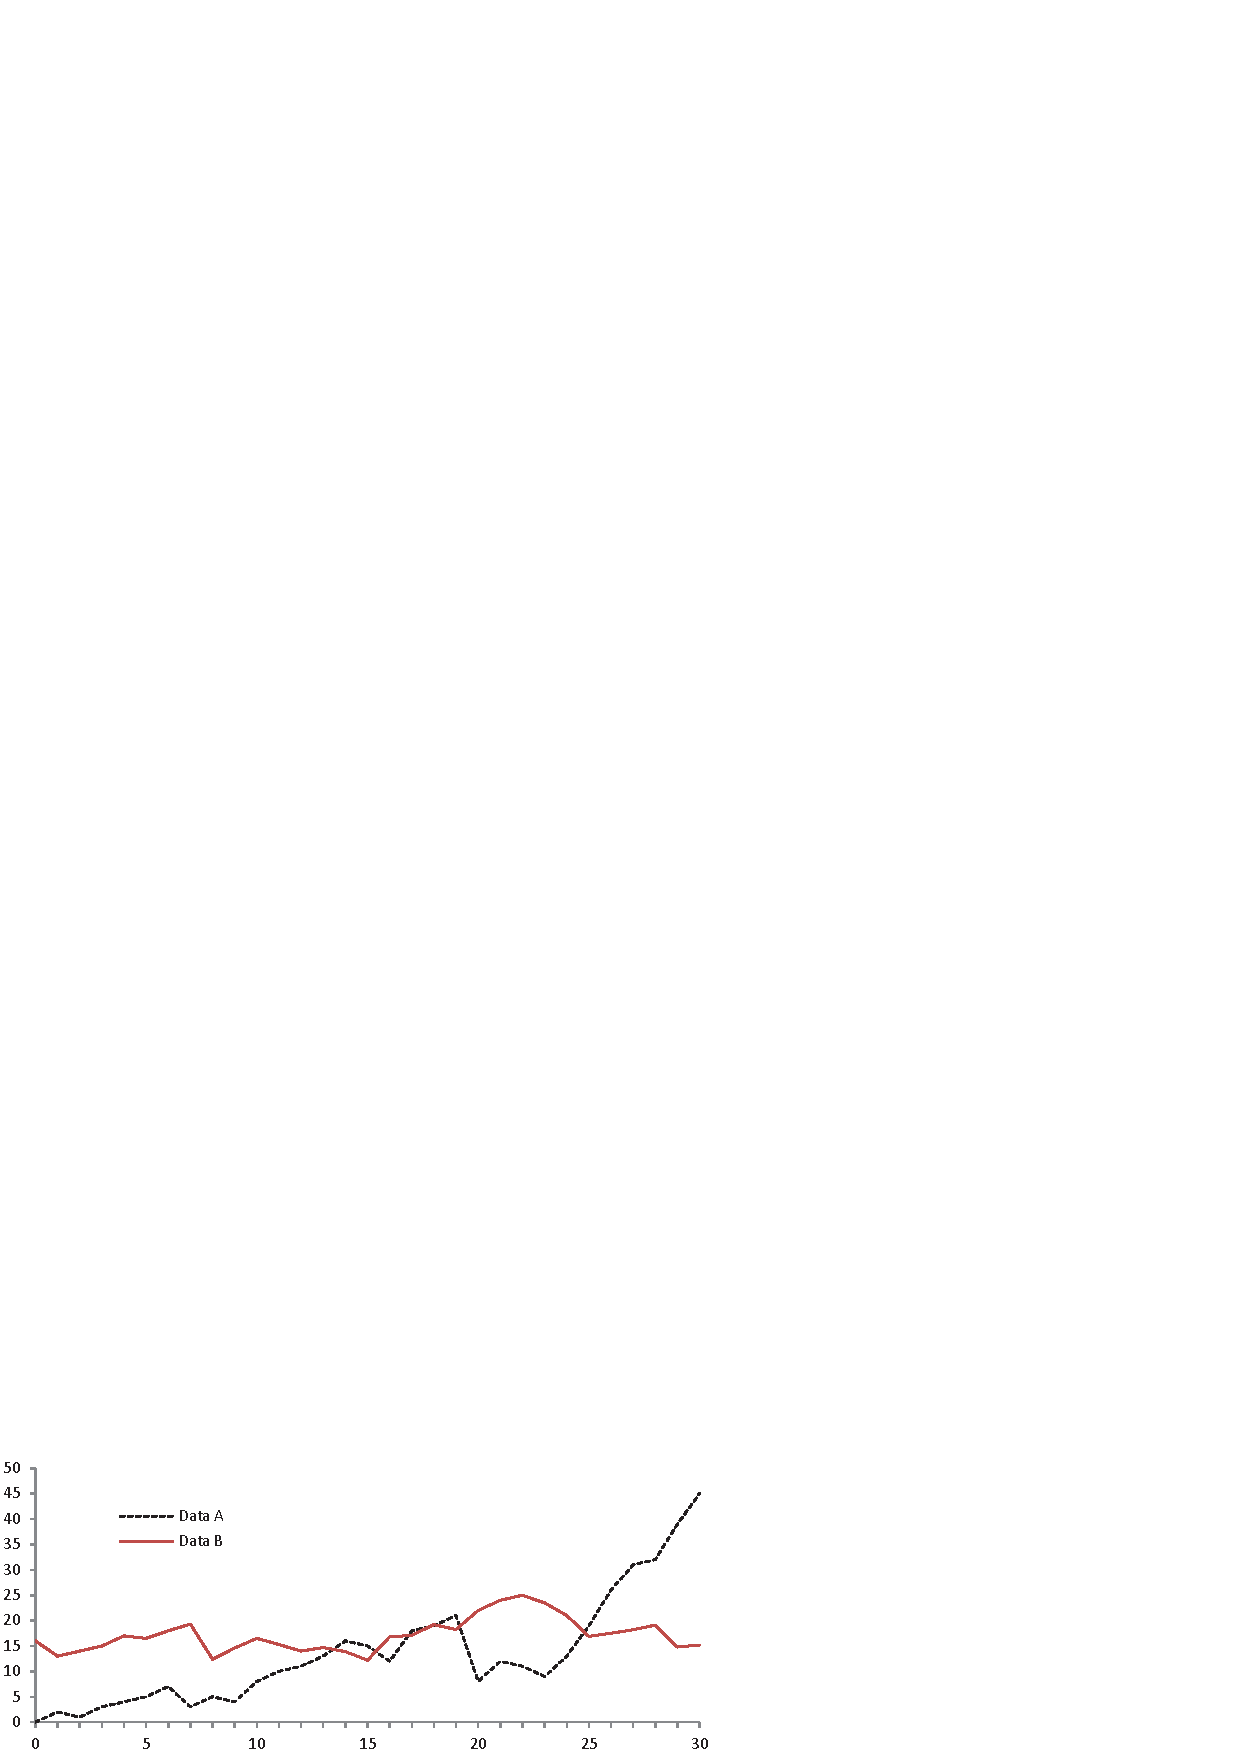
\includegraphics[width=0.8\columnwidth]{fig1.png}}
\caption{Example of a figure caption.}
\label{fig}
\end{figure}

Figure Labels: Use 8 point Times New Roman for Figure labels. Use words
rather than symbols or abbreviations when writing Figure axis labels to
avoid confusing the reader. As an example, write the quantity
``Magnetization'', or ``Magnetization, M'', not just ``M''. If including
units in the label, present them within parentheses. Do not label axes only
with units. In the example, write ``Magnetization (A/m)'' or ``Magnetization
\{A[m(1)]\}'', not just ``A/m''. Do not label axes with a ratio of
quantities and units. For example, write ``Temperature (K)'', not
``Temperature/K''.

\section*{Acknowledgment}

The preferred spelling of the word ``acknowledgment'' in America is without
an ``e'' after the ``g''. Avoid the stilted expression ``one of us (R. B.
G.) thanks $\ldots$''. Instead, try ``R. B. G. thanks$\ldots$''. Put sponsor
acknowledgments in the unnumbered footnote on the first page.

\printbibliography

% \section*{How to write the references}

% Please number citations consecutively within brackets \cite{b1}. The
% sentence punctuation follows the bracket \cite{b2}. Refer simply to the reference
% number, as in \cite{b3}---do not use ``Ref. \cite{b3}'' or ``reference \cite{b3}'' except at
% the beginning of a sentence: ``Reference \cite{b3} was the first $\ldots$''

% Number footnotes separately in superscripts. Place the actual footnote at
% the bottom of the column in which it was cited. Do not put footnotes in the
% abstract or reference list. Use letters for table footnotes.

% Unless there are six authors or more give all authors' names; do not use
% ``et al.''. Papers that have not been published, even if they have been
% submitted for publication, should be cited as ``unpublished'' \cite{b4}. Papers
% that have been accepted for publication should be cited as ``in press'' \cite{b5}.
% Capitalize only the first word in a paper title, except for proper nouns and
% element symbols.

% For papers published in translation journals, please give the English
% citation first, followed by the original foreign-language citation \cite{b6}.

% \begin{thebibliography}{00}
% \bibitem{b1} G. Eason, B. Noble, and I. N. Sneddon, ``On certain integrals of Lipschitz-Hankel type involving products of Bessel functions,'' Phil. Trans. Roy. Soc. London, vol. A247, pp. 529--551, April 1955.
% \bibitem{b2} J. Clerk Maxwell, A Treatise on Electricity and Magnetism, 3rd ed., vol. 2. Oxford: Clarendon, 1892, pp.68--73.
% \bibitem{b3} I. S. Jacobs and C. P. Bean, ``Fine particles, thin films and exchange anisotropy,'' in Magnetism, vol. III, G. T. Rado and H. Suhl, Eds. New York: Academic, 1963, pp. 271--350.
% \bibitem{b4} K. Elissa, ``Title of paper if known,'' unpublished.
% \bibitem{b5} R. Nicole, ``Title of paper with only first word capitalized,'' J. Name Stand. Abbrev., in press.
% \bibitem{b6} Y. Yorozu, M. Hirano, K. Oka, and Y. Tagawa, ``Electron spectroscopy studies on magneto-optical media and plastic substrate interface,'' IEEE Transl. J. Magn. Japan, vol. 2, pp. 740--741, August 1987 [Digests 9th Annual Conf. Magnetics Japan, p. 301, 1982].
% \bibitem{b7} M. Young, The Technical Writer's Handbook. Mill Valley, CA: University Science, 1989.
% \end{thebibliography}

% \appendices

% \section{Experimental data}
% \lipsum[1-4]
% \section{Theorem proofs}
% \lipsum[5-6]

% \vspace{12pt}
% \color{red}
% IEEE conference templates contain guidance text for composing and formatting conference papers. Please ensure that all template text is removed from your conference paper prior to submission to the conference. Failure to remove the template text from your paper may result in your paper not being published.

\end{document}
